Les systèmes d'interrogation de bases de données graphes visant les \emph{experts du domaine} plutôt que les experts dans des bases de données, suscitent un intérêt grandissant, car ce sont ces utilisateurs auxquels profite le plus l'information et qui sont les plus aptes à la transformer en connaissance.
Il est donc crucial de rendre ces systèmes plus conviviaux et accessibles aux utilisateurs sans compétences techniques avancées.
Malgré la puissance des langages d'interrogation comme \acrshort{sql}, \acrshort{sparql} ou encore \gls{cypher}, leur utilisation nécessite une compréhension de la structure des données et de leurs interactions.
Afin d'améliorer l'accessibilité à l'information sauvegardée dans ces \gls{sgbd}, la recherche sur les \gls{nli} a suscité beaucoup d'intérêt ces dernières années \cite{zhengQuestionAnsweringKnowledge2018,wangCrossdomainNaturalLanguage2019,xuMirrorNaturalLanguage2023,vargas-solarTranslatingDataScience2023,vargas-solarConversationalDataExploration2023}.
L'intérêt fondamental des interfaces en langage naturel réside dans la capacité à permettre aux utilisateurs de se concentrer sur la signification de leurs requêtes, plutôt que sur les mécanismes sous-jacents de recherche d'information.

Certains travaux se concentrent sur l'augmentation du pouvoir d'expression des requêtes, tandis que d'autres se concentrent sur l'indépendance par rapport au domaine.
Par exemple, dans~\cite{zhengQuestionAnsweringKnowledge2018}, les auteurs proposent d'utiliser des modèles binaires plutôt que des analyses sémantiques pour mieux comprendre les requêtes complexes, tandis que~\cite{wangCrossdomainNaturalLanguage2019} propose un \gls{nli} inter-domaines avec basé sur un étiquetage générique des questions proposées.
Plusieurs études \cite{zouNaturalLanguageQuestion2014,faderOpenQuestionAnswering2014,amsterdamerNaturalLanguageInterface2015} s'intéressent aux systèmes de questions-réponses, ou \gls{qa}, où les utilisateurs posent des questions en langage naturel sur une base de données \acrshort{rdf}.
Les requêtes d'agrégation sont examinées dans~\cite{huNaturalLanguageAggregate2018} : les auteurs proposent une méthode pour identifier automatiquement l'agrégation et la transformer en une instruction d'agrégation \acrshort{sparql}.
Les méthodes utilisées varient aussi considérablement.
Dans \cite{vargas-solarTranslatingDataScience2023}, les auteurs cherche à construire des requêtes pour l'analyse de données à partir d'une requête formulée en langage naturel.
\cite{vargas-solarConversationalDataExploration2023} propose un système pour l'exploration de donnée pour des graphes de propriétés en mode conversationnel.
Dans \cite{zafarFormalQueryGeneration2018,zhengQuestionAnsweringKnowledge2018,steinmetzNaturalLanguageQuestions2019}, les auteurs fondent leur approche sur des techniques de \gls{tal} avec l'extraction d'entités et des grammaires, tandis que dans \cite{utamaEndtoendNeuralNatural2018,wangCrossdomainNaturalLanguage2019}, ils utilisent des réseaux neuronaux.

Dans ce contexte, et en s'appuyant sur les méthodes de reconnaissances d'informations textuelles présentées dans les sections précédentes, on s'intéresse aux requêtes factuelles sur les instances d'une \emph{classe} \gls{rdf} avec deux objectifs principaux :
\begin{enumerate*}[label=(\roman*)]
    \item la facilité d'appliquer le système à divers domaines et
    \item la création de concepts d'interrogation plus complexes.
\end{enumerate*}
L'objectif est de concevoir un système d'interrogation permettant aux utilisateurs d'effectuer des recherches par facettes.
La recherche par facette consiste à filtrer une collection de données basée sur une unique collection d'individus par l'application de différents critères.
Il s'agit d'une requête conjonctive sur une unique classe appelée \emph{classe cible}.

Dans cette section, on présente la transformation d'une requête exprimée en langage naturel (nommée NL-query) en une requête de base de données (dénommée DB-query).
Cette proposition, faite dans \cite{amaviNaturalLanguageQuerying2020}, repose sur le formalisme établi dans la section~\ref{sec:update:pre:db}, page~\pageref{sec:update:pre:db} basé sur \gls{fol}.
En conséquence, ces requêtes peuvent être facilement traduites vers une modélisation graphe ou relationnelle en utilisant les langages de requêtes tels que \gls{sql}, \gls{sparql}, \gls{cypher}, etc.
On définit une formule logique $\phi$ ayant pour atomes :
\begin{enumerate}
    \item $P(t_1, \dots, t_n)$ où $P$ est un symbole de prédicat d'arité $n$ et $t_1, \dots, t_n$ sont des termes pouvant être des constantes ou des variables ;
    \item $\top$ (Vrai) / $\bot$ (Faux) ;
    \item $(t\ op\ \alpha)$ où $t$ est un terme, $\alpha$ est un terme ou un littéral et $op$ est un opérateur de comparaison.
\end{enumerate}
On rappelle qu'un fait est un atome $P(t_1, \dots, t_n)$ où l'ensemble des termes $t_1, \dots, t_n$ sont des constantes.
Par exemple, en \gls{rdf}, le fait $Book(Anatomy)$ signifie que $Anatomy$ est une instance de la classe \emph{Book}.
De manière similaire, $writtenBy(Anatomy, Bob)$, exprime que $Anatomy$ possède la valeur $Bob$ pour la propriété \textit{writtenBy}.
Le schéma de la base de données est représenté par un ensemble de prédicats $\mathcal{S}$ et l'instance de la base de données est représenté par l'ensemble de faits $\mathcal{D}$

\begin{definition}[NL-query]
    Une NL-query est une requête exprimée en langage naturel qui suit le format suivant : \textquote{Trouver des livres qui \dots} (en établissant \textbf{Book} comme \emph{classe cible}), \textquote{Quels médecins \dots} (en utilisant \textbf{Doctor} comme \emph{classe cible}), etc.
    Une requête valide sélectionne exclusivement des instances de  \emph{classe cible} (c'est-à-dire des nœuds du type donné) par l'intermédiaire de propriétés dont le domaine ou la portée est la \emph{classe cible} (c.-à-d. les arcs sortant ou entrant).
\end{definition}

Par exemple, en supposant que \emph{Book} est une \emph{classe cible}, une requête demandant des instances de \textquote{livres édités par le docteur Alice sur la cardiologie parut après 2018} est une requête acceptable.
Cependant, une requête demandant des exemples de \textquote{livres édités par le docteur Alice qui est cardiologue} n'est pas acceptable, car \textquote{est un cardiologue} n'est pas une propriété (ou une arête) de la \emph{classe cible} sélectionnée.
Si l'utilisateur souhaite identifier des médecins ayant rédigé un livre, il doit d'abord modifier la spécification de sa classe cible.
Plus simplement, on ne considère que des requêtes simples qui sont traduites en requêtes conjonctives de base de données identifiant des instances d'une classe particulière, même si elles fournissent également des informations sur les propriétés de ces instances.

\begin{definition}[DB-query]
    Une DB-query $q$ est une requête conjonctive sur un schéma donné $\mathcal{S}$ de la forme $R_0(u_0) \leftarrow \phi$ où $\phi = R_1(u_1) \dots  R_n(u_n), comp_1, \dots, comp_m$ où $n \geq 0$, $R_i$ sont des symboles de prédicats avec $0 \leq i \leq n$, $u_i$ est le tuple de termes de $R_i$ de longueur égale à l'arité de $R_i$ et $com_j$ sont des formules de comparaison qui incluent des variables trouvées dans au moins un tuple de $u_i$ avec $0 \leq j \leq m$.
    $head(q)$ (respectivement $body(q)$) représente la partie gauche de la règle, dénommée tête (respectivement la partie droite, dénommée corps) de $q$.
    $\mathbb{I}_q$ représente l'ensemble de réponses de $q$.

    Les réponses de $q$ sont des instanciations du tuple $u_0$ où l'ensemble des termes $t \in u_0$ sont des constantes.
    C-à-d. qu'il existe, pour chaque instanciation $I \in \mathbb{I}_q$, une surjection $h_I$ de $u_0$ vers $I$ (qui associe des variables à des constantes et une constante à elle-même) tel que : $\{R_1(h_t(u_1)), \dots, R_n(h_t(u_n))\} \subseteq \mathcal{D}$, la conjonction de tous les $h_I(comp_j)$ est évaluée à vrai (selon la sémantique habituelle des opérateurs $op$) et $h_I(u_0)= I$.

    % In this rule-based formalism, the union is expressed by allowing more than one rule with the same head.
    % For instance, 
    % $q(X) \leftarrow writtenBy(X, Bob)$ together with
    % $q(X) \leftarrow editedBy(X, Bob)$
    % express a query looking for documents written or edited by \textit{Bob}.
\end{definition}

\begin{example}
    La requête $NLQ_{run}$ en langage naturel suivante sera utilisée à titre d'exemple :
    \begin{displayquote}
        Livres intitulés \textquote{Principes de médecine}, écrits par Alice et Bob et dont le prix est inférieur à 30 euros.
    \end{displayquote}

    La figure~\ref{fig:nl-query:dep} montre l'arbre de dépendance pour une version simplifiée de $NLQ_{run}$.
    Dans cette requête, \textquote{Livre} représente la \emph{classe cible} : \emph{Book}.
    Cette requête se traduit dans la DB-query $Q_{run}$ suivante où \emph{:alice} et \emph{:bob} sont respectivement les identifiants en base d'Alice et Bob :
    \begin{equation*}
        \begin{split}
            Q(x) \leftarrow & Book(x), hasTitle(x, y_1), writtenBy(x, y_2), Person(y_2), writtenBy(x, y_3), Person(y_3),                      \\
                            & hasPrice(x, y_4), (y_1 = \text{"Principes de médecine"}), (y_2= \text{:alice}), (y_3 = \text{:bob}), (y_4 < 30)
        \end{split}
    \end{equation*}
\end{example}

\begin{figure}[htb]
    \tiny
    \centering
    \begin{adjustbox}{width=\linewidth}
        \begin{dependency}[theme=simple, edge horizontal padding=5ex, edge unit distance=1em, column sep=2em]
            \begin{deptext}
                Livres \& écrits \& par \& Alice \& et \& Bob \& et \& dont \& le \& prix \& est \& inférieur \& à \& 30 \& euros \\
                NOUN \& VERB \& ADP \& PROPN \& CCONJ \& PROPN \& CCONJ \& PROPN \& DET \& NOUN \& AUX \& ADJ \& ADP \& NUM \& NOUN \\
            \end{deptext}

            \deproot[edge height=15ex]{1}{ROOT}
            \depedge{1}{2}{acl}
            \depedge{2}{4}{auoblx}
            \depedge{4}{3}{case}
            \depedge{4}{6}{conj}
            \depedge{6}{5}{cc}
            \depedge[segmented edge, edge height=13ex]{2}{12}{conj}
            \depedge[segmented edge, edge height=10ex]{12}{7}{cc}
            \depedge{12}{10}{nsubj}
            \depedge{12}{11}{cop}
            \depedge{10}{8}{nmod}
            \depedge{10}{9}{det}
            \depedge{12}{15}{obl}
            \depedge{15}{13}{case}
            \depedge{15}{14}{nummod}
        \end{dependency}
    \end{adjustbox}
    \caption[Arbre de dépendance d'une version simplifiée de $NLQ_{run}$]{Arbre de dépendance d'une version simplifiée de $NLQ_{run}$ obtenu avec \gls{spacy}}
    \label{fig:nl-query:dep}
\end{figure}

\subsection{Extraction d'entités}

En s'appuyant sur les sections précédentes, l'ensemble des classes présentes dans la base de données peuvent être représentées par un lexique.
Dans l'exemple de $NLQ_{run}$, on suppose que l'on a un lexique de \emph{Personne} qui a pour valeur les identifiants des individus associés au nom, prénom, etc. de chaque personne.
Ainsi, l'ensemble des individus de la base peuvent être reconnus et associé directement à la classe (correspondant au type de l'entité).
Un lexique des classes cible disponible et un lexique des champs/propriété dans la base sont aussi construit.
Ces lexiques nécessitent généralement une intervention humaine pour compléter la liste des synonymes pour ne pas uniquement dépendre du nom de la classe.
Pour identifier les dates et les nombres (ex : 30 euros), on utilise un ensemble de grammaire locale.
Les \emph{textes libres}, comme le titre dans $NLQ_{run}$, sont extrait à l'aide d'un \gls{crf} appris sur un jeu de donnée généré en utilisant un \gls{dsl}.
L'exemple~\ref{ex:nl-query:simpleEnts} montre les entités extraites pour la requête $NLQ_{run}$.

\begin{example}
    \label{ex:nl-query:simpleEnts}
    Ci-dessous nous présentons la requête $NLQ_{run}$ avec les entités extraites dans des rectangles.
    Chaque entité est numérotée.
    Les entités \ref{nl-query:e1}, \ref{nl-query:e3}, \ref{nl-query:e4} et \ref{nl-query:e5} sont extraite par l'intermédiaire de lexiques.
    L'entité \ref{nl-query:e6} est obtenu en utilisant une grammaire locale et \ref{nl-query:e2} et extraite à l'aide d'un \gls{crf}.

    \begin{displayquote}
        \fbox{Livres~\tiny{1}} intitulés \fbox{\textquote{Principes de médecine}~\tiny{2}} écrits par \fbox{Alice~\tiny{3}} et \fbox{Bob~\tiny{4}} et dont le \fbox{prix~\tiny{5}} est \fbox{inférieur à~\tiny{6}} \fbox{30 euros~\tiny{7}}.
    \end{displayquote}

    \noindent
    On a donc les entités suivantes :
    \begin{multicols}{2}
        \begin{enumerate}[label=$E_{\arabic*}$]
            \item \label{nl-query:e1} $= (Book, Class)$
            \item \label{nl-query:e2} $= (\text{Principes de médecine}, Text)$
            \item \label{nl-query:e3} $= (:alice, Person)$
            \item \label{nl-query:e4} $= (:bob, Person)$
            \item \label{nl-query:e5} $= (hasPrice, Attribut)$
            \item \label{nl-query:e6} $= (<, Operator)$
            \item \label{nl-query:e7} $= (30, Number)$
        \end{enumerate}
    \end{multicols}

    Pour des raisons de lecture, on ne représente pas la notation des ensembles de valeurs et de types.
    Ici, chaque entité n'a qu'une seule valeur et chaque valeur est associée à un unique type.
    Dans la pratique, il serait possible d'avoir plusieurs valeurs ou types à cause de l'ambiguïté.
    Ainsi, si $p_1$ et $p_2$ sont deux personnes dans la base qui se prénomme Alice, alors on aurait :
    \begin{equation*}
        E_3 = (\{p_1, p_2\}, \{Personne\}, \langle p_1 \mapsto \{Personne\}, p_2 \mapsto \{Personne\} \rangle)
    \end{equation*}
\end{example}

L'extraction des associations \emph{classe cible} -- attributs (c.-à-d. des arêtes dans le graphe) se fait par contextualisation.
Comme discuté dans la section~\ref{sec:tal:ctx}, cette dernière peut s'opérer par extraction de marqueur de contexte (dans $NLQ_{run}$, on peut identifier les marqueurs \textquote{intitulés} et \textquote{écrits par}) ou en utilisant un \gls{crf}.
Ici, on utilise des \acrshortpl{crf} pour les attributs génériques et l'ensemble de règles donné dans la section~\ref{sec:tal:ctx:rule} pou identifier le lien entre une entité correspondante à un attribut (ex : \ref{nl-query:e5} \textquote{prix}) et l'entité correspondante à la valeur de l'attribut (ex : \ref{nl-query:e6} \textquote{30 euros}).
Dans $NLQ_{run}$, on remarque la présence d'un opérateur \textquote{inférieur à}.
Un opérateur est un modificateur (comme les contextes) qui vient enrichir la valeur (contrairement au type pour les contextes) d'une entité.
Les opérateurs sont identifiés comme les contextes, on utilise un lexique pour le marqueur et la détection des liens avec une entité est effectué par l'ensemble de règles sur l'arbre de dépendances (figure~\ref{fig:nl-query:dep}) utilisées pour la contextualisation et listée dans la section~\ref{sec:tal:ctx:rule}.
Il est possible d'avoir des opérateurs sans valeurs associées et qui peuvent être liée à un attribut de la \emph{classe cible}.
Par exemple, c'est le cas pour les opérateurs \textquote{est vide} et \textquote{est rempli}.

\begin{example}
    \label{ex:nl-query:enrichEnts}
    Pour $NLQ_{run}$, l'association entre les entités \ref{nl-query:e5} \textquote{prix} et \ref{nl-query:e6} \textquote{30 euros} est réalisé en deux temps.
    On commence par associer l'opérateur \textquote{inférieur à} à l'entité \ref{nl-query:e7}.
    On obtient alors l'annotation suivante :
    \begin{displayquote}
        \fbox{Livres~\tiny{1}} intitulés \fbox{\textquote{Principes de médecine}~\tiny{2}} qui ont été écrits par \fbox{Alice~\tiny{3}} et \fbox{Bob~\tiny{4}} et dont le \fbox{prix~\tiny{5}} est \fbox{inférieur à 30 euros~\tiny{7}}.
    \end{displayquote}
    Ensuite, on identifie que l'entité \ref{nl-query:e7} ($<30$) est associé à l'attribut pointé par l'entité \ref{nl-query:e5} ($hasPrice$).
    Seule les types associée au schéma de la base sont gardés ainsi, les types \emph{Text}, \emph{Number} et \emph{Date} sont filtrés.
    On obtient alors l'entité enrichie \ref{nl-query:e7} $= (30, \{Number, hasPrice\}, <)$.
    \begin{multicols}{2}
        \begin{enumerate}[label=$E_{e\arabic*}$]
            \item \label{nl-query:ee1} $= \{(Book, \{Class\}, =)\}$
            \item \label{nl-query:ee2} $= \{(\text{"Principes de médecine"}, \{Title\}, =)\}$
            \item \label{nl-query:ee3} $= \{(\text{:alice}, \{Person, Author\}, =)\}$
            \item \label{nl-query:ee4} $= \{(\text{:bob}, \{Person, Author\}, =)\}$
            \item \label{nl-query:ee5} $= \{(30, \{hasPrice\}, <)\}$
        \end{enumerate}
    \end{multicols}
\end{example}

\subsection{Construction de DB-query à partir d'entités enrichies}

\SetKwFunction{GetNewVar}{getNewVar}
\SetKwFunction{BuildAtom}{buildAtom}
\SetKwFunction{BuildAtomOP}{buildAtomOP}
\SetKwFunction{BuildNewQuery}{buildNewQuery}

Après analyse de la NL-query et l'extraction de l'ensemble $\mathcal{E}$ des entités enrichies, la DB-query est construite à l'aide de la procédure~\ref{algo:nl-query}.
L'algorithme commence par considérer l'entité $E_{e1}$ (ligne~\ref{algo:nl-query:target}) qui a un rôle spécial puisqu'elle spécifie la \emph{classe cible} qui est interrogée.
La requête est initialisée avec un corps composé d'un unique atome sur le prédicat associé à la classe cible.
La procédure \BuildAtom est responsable de la construction d'un atome pour la requête en cours de construction.
Le symbole du prédicat à utiliser dans la construction d'un atome est trouvé via la valeur de l'entité $E_{e1}$.
Dans l'exemple~\ref{ex:nl-query:simpleEnts}, \emph{Book} est la valeur de \ref{nl-query:ee1} et le nom du prédicat unaire associé.
Dans notre cas, l'atome $A_0$ est $Book(x)$.
Remarquons que l'algorithme~\ref{algo:nl-query} ne construit que des requêtes dont les réponses sont des identifiants de livres (c'est-à-dire des instanciations de $x$).
Dans cet exemple, la requête initiale est donc : $q(x) \leftarrow Book(x)$.

\begin{procedure}[htb]
    \caption{entitiesToQueries($\mathcal{E}$)}
    \label{algo:nl-query}

    %\Input{$\mathcal{E}$ an enriched entity set $\{E_{e0}, E_{e1}, \dots\}$}
    %\Output{$\mathcal{Q}$ a set of query rules, i.e., the DB-query with one or more rules}

    $\mathcal{Q} \gets \emptyset$ \;
    \ForEach{entité enrichie $E \in \mathcal{E}$}{
        \eIf{$E$ is $E_{e1}$\label{algo:nl-query:target}}{
            $\{ (value, type, op) \} \gets E$ \;
            $A_0 \gets \BuildAtom(value, x)$ \tcp*[l]{Construit le premier atome du corps de la requête}
            $\mathcal{Q} \gets \{ Q(x) \leftarrow A_0 \}$ \;
        }{
            $Parts \gets \emptyset$ \tcp*[l]{Ensemble des listes d'atomes. Chaque $l \in Parts$ est une liste d'atomes dont la conjonction doit être ajoutée au corps de la requête.}

            \ForEach{$(value, op) \in E$\label{algo:nl-query:ent-start}}{
                \ForEach{$type \in E(value)$\label{algo:nl-query:types}}{
                    $y \gets \GetNewVar$ \;
                    $part \gets \{\BuildAtomOP(value, y, opval), \BuildAtom(type, y)\}$ \;
                    $Parts \gets Parts \cup \{part\}$\label{algo:nl-query:part} \;
                }
            }\label{algo:nl-query:ent-end}

            $\mathcal{Q}' \gets \emptyset$ \;
            \ForEach{requête $q \in \mathcal{Q}$\label{algo:nl-query:queries}}{
                \ForEach{$part \in Parts$}{
                    $q' = \BuildNewQuery(q, part)$ \label{algo:nl-query:query} \;
                    $\mathcal{Q}' \gets \mathcal{Q}' \cup \{q'\}$ \;
                }
            }
            $\mathcal{Q} \gets \mathcal{Q}'$ \;
        }
    }
    \Return $\mathcal{Q}$ \;
\end{procedure}

Les lignes~\ref{algo:nl-query:ent-start} à \ref{algo:nl-query:ent-end} de la procédure~\ref{algo:nl-query} traite les entités $E_e$ enrichies.
On commence par construire pour chaque valeur de l'entité une variable avec la fonction \GetNewVar et on construit la formule de comparaison correspondant à l'opérateur entre la variable et la valeur à l'aide de la fonction \BuildAtomOP.
Pour chaque type associé à la valeur ($E(value)$, ligne~\ref{algo:nl-query:types}), on construit les atomes correspondants.
La fonction \BuildAtom est utilisée pour construire les atomes qui seront ajoutés à $body(q)$.
Notez que \BuildAtom associe à chaque type, le symbole de prédicat correspondant et construit l'atome en prenant en compte l'emplacement de la valeur de l'entité (variable $y$) dans l'atome.
Dans les prédicats binaires, $x$ est toujours l'autre variable.
Si, dans $E_e$, il y a plus d'une valeur, alors l'entité est ambiguë, soit parce qu'elle a été extraite par un lexique et que le lexème est ambiguë soit c'est une entité obtenue après prise en compte de la conjonction de coordination \textit{or}.
On matérialise l'ambiguïté par une union de requête.
Pour ce faire, la procédure~\ref{algo:nl-query} divise les valeurs de $E_e$ en sous partie de la requête.
Chaque $l \in Parts$ est un ensemble d'atomes à ajouter au corps de la requête en cours de construction.
Dans la boucle à la ligne~\ref{algo:nl-query:queries} on calcule le produit cartésien entre les requêtes déjà construites et les parties correspondantes à chaque valeur de l'entité $E_e$.
C'est-à-dire que si $E_e$ possède deux valeurs possibles, on aura le double de requêtes qui seront construite.

D'après l'exemple~\ref{ex:nl-query:enrichEnts}, \ref{nl-query:ee3} a deux types : \emph{Person} et \emph{Author}.
Ainsi, sur la ligne~\ref{algo:nl-query:part} on ajoute l'ensemble $\{ Person(y_2),$ $writtenBy(x, y_2),$ $(y_2= \text{:alice}) \}$ à $Parts$ et à la ligne~\ref{algo:nl-query:query} la requête construite est :
\begin{equation*}
    \begin{split}
        q(x) \leftarrow & Book(x), Person(y_2), writtenBy(x, y_2), (y_2= \text{:alice})
    \end{split}
\end{equation*}

Le résultat obtenu avec l'entité \ref{nl-query:ee4} est similaire.
Pour \ref{nl-query:ee2} et \ref{nl-query:ee5}, un seul prédicat est construit, car les valeurs n'ont qu'un seul type associé.
Par exemple, \ref{nl-query:ee2} donne lieu à l'ensemble $\{ hasTitle(x, y_1),$ $(y_1 = \text{"Principes de médecine"}) \}$.
Le traitement de l'entité \ref{nl-query:ee5} construit la comparaison $y_4 < 30$.
Après avoir pris en compte toutes les entités, la procédure~\ref{algo:nl-query} renvoie l'ensemble $\mathcal{Q}$ qui forme la DB-query suivante :
\begin{equation*}
    \begin{split}
        Q(x) \leftarrow & Book(x), hasTitle(x, y_1), writtenBy(x, y_2), Person(y_2), writtenBy(x, y_3), Person(y_3),                      \\
                        & hasPrice(x, y_4), (y_1 = \text{"Principes de médecine"}), (y_2= \text{:alice}), (y_3 = \text{:bob}), (y_4 < 30)
    \end{split}
\end{equation*}

Cependant, considérons qu'il existe une ambiguïté sur l'entité \ref{nl-query:ee3} avec les valeurs \emph{:alice1} et \emph{:alice2} tel que \ref{nl-query:ee3} $= \{(\text{:alice1},$ $\{Person, Author\}, =),$ $(\text{:alice2},$ $\{Person, Author\}, =)\}$.
La procédure~\ref{algo:nl-query} (lignes~\ref{algo:nl-query:ent-start} à~\ref{algo:nl-query:ent-end}) produit deux sous requête à partir de la même entité, à savoir :
\begin{enumerate*}[label=(\roman*)]
    \item $part_1 = \{ Person(y_2),$ $writtenBy(x, y_2),$ $(y_2 = \text{:alice1}) \}$ et
    \item $part_2 = \{ Person(y_2),$ $writtenBy(x, y_2),$ $(y_2 = \text{:alice2}) \}$.
\end{enumerate*}
Ensuite, à la ligne~\ref{algo:nl-query:queries}, chaque sous requête est considérée séparément et la requête $Q$ est remplacée par deux nouvelles requêtes.
À la fin de la procédure, $\mathcal{Q}$ est une requête DB-query composée de deux règles :
\begin{equation*}
    \begin{split}
        Q(x) \leftarrow & Book(x), hasTitle(x, y_1), writtenBy(x, y_2), Person(y_2), writtenBy(x, y_3), Person(y_3),                       \\
                        & hasPrice(x, y_4), (y_1 = \text{"Principes de médecine"}), (y_2= \text{:alice1}), (y_3 = \text{:bob}), (y_4 < 30) \\
        Q(x) \leftarrow & Book(x), hasTitle(x, y_1), writtenBy(x, y_2), Person(y_2), writtenBy(x, y_3), Person(y_3),                       \\
                        & hasPrice(x, y_4), (y_1 = \text{"Principes de médecine"}), (y_2= \text{:alice2}), (y_3 = \text{:bob}), (y_4 < 30)
    \end{split}
\end{equation*}

Enfin, considérons la NL-query \textit{livres édités ou écrits par Alice} comprenant l'entité enrichie $E_{e2} = \{(\text{:alice}, \{Person, Author\}, =), (\text{:alice}, \{Person, Editor\}, =)\}$.
Les ensembles construits à la ligne~\ref{algo:nl-query:part} sont :
\begin{enumerate*}[label=(\roman*)]
    \item $part_1 = \{ Person(y),$ $writtenBy(x, y),$ $(y = \text{:alice}) \}$ et
    \item $part_2 = \{ Person(y),$ $editedBy(x, y),$ $(y = \text{:alice}) \}$.
\end{enumerate*}
On obtient alors la DB-query suivante :
\begin{equation*}
    \begin{split}
        Q(x) \leftarrow & Book(x), Person(y), writtenBy(x, y), (y = \text{:alice}) \\
        Q(x) \leftarrow & Book(x), Person(y), editedBy(x, y), (y = \text{:alice})
    \end{split}
\end{equation*}

\subsection{Évaluation}
Le système est évalué sur un cas concret impliquant une instance de la \glsreset{ged}\gls{ged} d'\gls{ennov}.
Dans cette configuration, les métadonnées des documents sont regroupées et indexées automatiquement dans des lexiques.
Après l'extraction des différentes entités, une phase de post-traitement est ajoutée pour éliminer les incohérences éventuelles.
Par exemple, cette phase vérifie si une entité identifiée comme un champ personne est bien associé à un identifiant valide de personne.
Si ce n'est pas le cas, la condition est supprimée.
Cette étape de post-traitement permet ainsi de rectifier d'éventuelles erreurs survenues lors de l'extraction et de la contextualisation des entités.

\begin{figure}[htb]
    \centering
    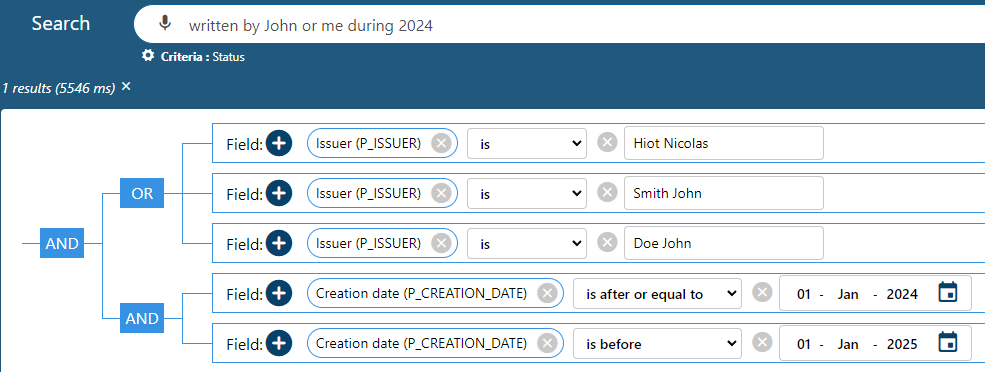
\includegraphics[width=\textwidth]{these/part_2/chapter_2/imgs/ui-nlsearch-compress.png}
    \caption[Interface utilisateur pour la recherche en langage naturel]{Interface utilisateur et exemple de résultat pour la recherche en langage naturel}
    \label{fig:nl-query:ui}
\end{figure}

La figure~\ref{fig:nl-query:ui} présente l'interface utilisateur ainsi qu'un exemple de requête en anglais : \enquote{written by John or me during 2024}.
Le résultat de la recherche n'est pas présent sur cette figure.
Pour aider l'utilisateur à comprendre la requête qui a été formulée, celle-ci est représentée sous forme d'un arbre, tel que présenté sur la figure.
Dans la requête, on observe par exemple l'utilisation de la conjonction \textquote{ou} entre \emph{Nicolas} et \emph{John} ainsi que l'ambiguïté du prénom \emph{John}.
De plus, la date exprimée par \enquote{during 2024} est convertie en une plage de valeur, créant ainsi deux conditions : $>= 2024$ et $<2025$.
Dans cette implémentation, nous utilisons la bibliothèque \gls{duckling}\footnote{\url{https://github.com/facebook/duckling}} pour extraire les entités détectables par des grammaires locales telles que les dates, les nombres, les adresses e-mail, etc.

\begin{table}[htb]
    \centering
    \begin{tabular}{r|cccc}
                         & Précision      & Rappel         & Mesure F1      & Support    \\
        \hline
        \hline
        object type      & \num{0,600764} & \num{0,990551} & \num{0,747919} & \num{ 635} \\
        person           & \num{0,654574} & \num{0,734513} & \num{0,692244} & \num{1130} \\
        field            & \num{0,292157} & \num{0,977049} & \num{0,449811} & \num{ 305} \\
        type             & \num{0,330645} & \num{0,976190} & \num{0,493976} & \num{ 168} \\
        unit             & \num{0,638254} & \num{0,987138} & \num{0,775253} & \num{ 311} \\
        status           & \num{0,575368} & \num{0,970543} & \num{0,722447} & \num{ 645} \\
        \hline
        time             & \num{0,941496} & \num{0,916618} & \num{0,928890} & \num{1703} \\
        title            & \num{0,577215} & \num{0,679920} & \num{0,624372} & \num{1006} \\
        \hline
        application date & \num{0,888889} & \num{0,522105} & \num{0,657825} & \num{ 475} \\
        archive date     & \num{0,899135} & \num{0,715596} & \num{0,796935} & \num{ 436} \\
        creation date    & \num{0,698080} & \num{0,804829} & \num{0,747664} & \num{ 497} \\
        expiration date  & \num{0,814655} & \num{0,675000} & \num{0,738281} & \num{ 280} \\
        issuer           & \num{0,724954} & \num{0,597598} & \num{0,655144} & \num{ 666} \\
        signatories      & \num{0,708738} & \num{0,478166} & \num{0,571056} & \num{ 458} \\
        \hline
        Total            & \num{0,667495} & \num{0,787558} & \num{0,685844} & \num{8715}
    \end{tabular}
    \caption{Score obtenu pour l'extraction d'entités pour la recherche en langage naturel}
    \label{tab:nl-query:result}
\end{table}

La table~\ref{tab:nl-query:result} présente les résultats de l'évaluation sur un corpus synthétique de test.
Le corpus de test a été généré en utilisant le même  \gls{dsl} que celui utilisé pour les données d'entraînement des \acrshortpl{crf}.
La première section (de \emph{object type} à \emph{unit}) concerne les entités extraites à l'aide de lexiques.
Les entités \emph{time} sont extraites en utilisant des grammaires locales (via \gls{duckling}), tandis que les entités \emph{title} sont extraites à l'aide d'un \gls{crf}.
La section suivante (de \emph{application date} à \emph{signatories}) concerne les entités contextualisées, où les dates sont extraites à partir de l'entité \emph{time} et les entités \emph{issuer/signatories} sont obtenues à partir de l'entité \emph{person}.

De manière générale, on observe que les lexiques donnent un très bon rappel (supérieur à \num{0.9}), mais une précision plus faible, en particulier pour les entités \emph{field} et \emph{type}.
Cela s'explique par le manque de filtrage sur les lexiques : dans cette version, nous ne filtrons pas les lexèmes trop génériques.
Les entités \emph{field} et \emph{type} sont deux cas particuliers où les lexèmes associés à chaque valeur peuvent être longs.
Pour l'entité \emph{title}, il est difficile d'annoter correctement les bornes de l'entité en raison de la longueur de la séquence et de la grande variabilité dans les titres.
L'entité \emph{time} est la mieux annotée avec une mesure F1 de \num{0.93}.
En ce qui concerne la contextualisation, on remarque que les dates sont correctement classifiées à \SI{70}{\percent}.
En revanche, pour les entités \emph{issuer} et \emph{signatories}, le système a du mal à classifier correctement les personnes.
Le \gls{crf} associé s'appuie sur les entités \emph{person} extraites précédemment et dépend donc de leur qualité, qui est parmi les trois plus faibles, avec seulement \num{0.69} pour la mesure F1.

\paragraph{}
Une des problématiques majeures rencontrées dans ce type d'application est le temps de traitement.
L'extraction est effectuée par un enchaînement séquentiel de composants exécuté avec l'écosystème \gls{ray} sur une machine équipée de \SI{4}{vCPU} et \SI{16}{\giga\byte} de mémoire primaire.
Nous utilisons les modèles \gls{spacy} \textsf{en\_core\_web\_md} (version 3.7.1) pour l'anglais et \textsf{fr\_core\_news\_md} (version 3.7.0) pour le français.
Le temps moyen nécessaire pour l'analyse du texte, les vérifications de cohérence par rapport à la base pour le post-traitement et l'exécution de la recherche sur un core \gls{solr} est d'environ \SI{2.5}{\second}.
Bien que ce temps d'exécution soit acceptable, il demeure élevé, en particulier en raison des vérifications qui génèrent plusieurs requêtes en base et sont traitées de manière séquentielle.
En plus de traiter les vérifications de façon concurrente, il serait possible de considérer l'enchaînement des composants comme un graphe acyclique orienté ou \gls{dag} en anglais plutôt que comme une séquence, afin de calculer certaines étapes en parallèle.

Une autre problématique de cette approche est que les différents composants du système sont entraînés individuellement.
Il pourrait être intéressant d'envisager d'entraîner les \acrshortpl{crf} à partir des annotations que les composants précédents sont capables d'extraire, plutôt que de les entraîner à partir de données correctement annotées.

\FloatBarrier
\subsection{Construction de graphique}

\begin{figure}[htb]
    \centering
    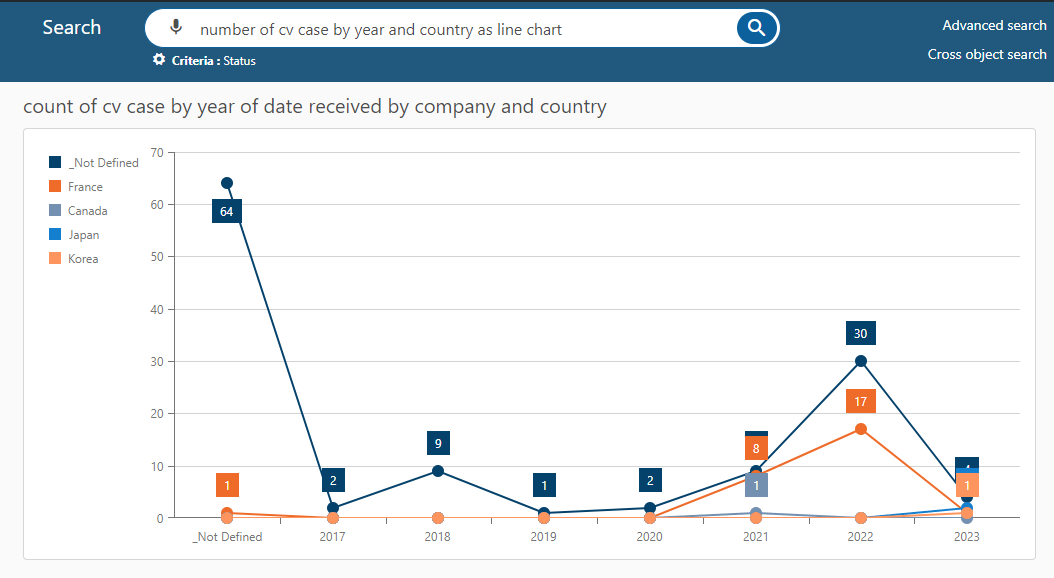
\includegraphics[width=\textwidth]{these/part_2/chapter_2/imgs/ui-dashboard-compress.png}
    \caption[Interface utilisateur pour la construction de graphique]{Interface utilisateur et exemple de résultat pour la construction de graphique à partir d'une requête en langage naturel}
    \label{fig:nl-query:dashboard-ui}
\end{figure}

Pour aller plus loin, nous proposons de permettre la création de graphiques à partir d'une requête en langage naturel.
L'idée est de permettre à un utilisateur de construire simplement un graphique à partir des données présentes dans la base.
Chaque graphique est construit à partir des champs d'une seule table.
La figure~\ref{fig:nl-query:dashboard-ui} illustre le résultat de cette fonctionnalité dans l'interface utilisateur.
Par exemple, dans cette illustration, nous recherchons l'évolution du nombre de cas de cosmétovigilance par année de réception de l'entreprise et par pays.

Pour cela, on commence par identifier le type de graphique (\emph{chart type}), si on ne le trouve pas, on détermine le type automatiquement en fonction du nombre d'axes sélectionnés.
Ensuite, on identifie les différents axes du graphique : \emph{value axis} pour les ordonnées, \emph{x axis} pour l'axe des abscisses et \emph{y axis} pour le second axe utilisé pour construire plusieurs courbes dans l'exemple de la figure~\ref{fig:nl-query:dashboard-ui}.
Pour chaque axe, on identifie l'étiquette (\emph{value label}, \emph{x label} et \emph{y label}) si elle est fournie, le champ de la table utilisé pour l'axe (\emph{field}) la fonction d'agrégation pour les valeurs (\emph{axis aggregate}, moyenne, somme, etc) et le modificateur (\emph{axis modifier}, par exemple, pour une date, on peut demander seulement le mois ou l'année).
Pour finir, on cherche la table à utiliser, si elle n'est pas spécifiée dans la requête de l'utilisateur, on cherche la table la plus petite qui contient les champs identifiés.
Ici on ne s'intéresse qu'à l'extraction des entités, mais un filtrage est effectué après l'extraction pour s'assurer que le graphique construit est cohérent, permettant de rejeter certaines ambiguïtés.

\begin{table}[htb]
    \centering
    \begin{tabular}{r|cccc}
                       & Précision      & Rappel         & Mesure F1      & Support    \\
        \hline
        \hline
        axis aggregate & \num{0,910714} & \num{0,980769} & \num{0,944444} & \num{ 156} \\
        axis modifier  & \num{0,432500} & \num{0,994253} & \num{0,602787} & \num{ 174} \\
        chart type     & \num{0,936747} & \num{1,000000} & \num{0,967341} & \num{ 311} \\
        table          & \num{0,691983} & \num{0,716157} & \num{0,703863} & \num{ 229} \\
        field          & \num{0,292157} & \num{0,977049} & \num{0,449811} & \num{ 305} \\
        \hline
        value axis     & \num{0,940461} & \num{0,990560} & \num{0,964860} & \num{1483} \\
        x axis         & \num{0,894330} & \num{0,973807} & \num{0,932378} & \num{1069} \\
        y axis         & \num{0,822669} & \num{0,813743} & \num{0,818182} & \num{ 553} \\
        value label    & \num{0,894886} & \num{0,875000} & \num{0,884831} & \num{ 360} \\
        x label        & \num{0,915541} & \num{1.000000} & \num{0,955908} & \num{ 271} \\
        y label        & \num{0,913043} & \num{0,777778} & \num{0,840000} & \num{ 162} \\
        \hline
        Total          & \num{0,785912} & \num{0,918128} & \num{0,824037} & \num{5073}
    \end{tabular}
    \caption[Score obtenu pour l'extraction d'entités pour la construction de graphiques]{Score obtenu pour l'extraction d'entités pour la construction de graphiques à partir d'une requête en langage naturel}
    \label{tab:nl-query:result-dashboard}
\end{table}

La table~\ref{tab:nl-query:result-dashboard} présente les résultats obtenus.
Le premier groupe d'entités (de \emph{axis aggregate} à \emph{tables}) est extrait à partir de lexiques te le second groupe (de \emph{value axis} à \emph{y label}) sont extrait à partir de \acrshortpl{crf}.
L'extraction des axes (\emph{value axis}, \emph{x axis}, \emph{y axis}) se repose sur les entités : \emph{axis aggregate}, \emph{axis modifier}, \emph{chart type}, \emph{table} et \emph{fields}.
Les étiquettes des axes (\emph{value label}, \emph{x label}, \emph{y label}) se basent sur l'extraction des entités : \emph{value axis}, \emph{x axis} et \emph{y axis}.

On identifie, pour les lexiques \emph{axis modifier} et \emph{field}, une problématique similaire à celle évoquée pour la recherche en langage naturel où les lexèmes sont assez génériques.
On obtient donc une bonne couverture (rappel de \num{0,99}) mais une précision assez faible (\num{0,36}).
La contextualisation s'appuie ici sur un plus grand nombre d'entités, ce qui augmente la qualité générale (F1 de \num{0,69} pour la recherche et \num{0,90} pour la construction de graphique).
De plus, les requêtes sont plus structurées avec un ordre clair des axes (\emph{value} $\to$ \emph{x} $\to$ \emph{y}), n'ont pas de chevauchement possible (contrairement aux contextes de dates ou de personne) et sont composées d'un plus faible nombre d'entités.

\FloatBarrier
